\documentclass{article}
	
\usepackage[margin=1in]{geometry}		% For setting margins
\usepackage{amsmath}				% For Math
\usepackage[]{amssymb}
\usepackage{amsmath}
\usepackage{gensymb}
\usepackage{fancyhdr}				% For fancy header/footer
\usepackage{graphicx}				% For including figure/image
\usepackage{cancel}					% To use the slash to cancel out stuff in work
\usepackage{wasysym}                % For cent symbol
\usepackage{needspace}              % To force item to next page

%%%%%%%%%%%%%%%%%%%%%%
% Set up fancy header/footer
\pagestyle{fancy}
\fancyhead[RO,R]{{\large\textbf{PHYS-102}}}
\fancyhead[LO,L]{\large{\textbf{Ch 20 Problem Set}}}
% \fancyhead[CO,C]{\large{\textbf{Part 1}}}
% \fancyhead[RO,R]{\today}
\fancyfoot[LO,L]{}
\fancyfoot[CO,C]{\thepage}
\fancyfoot[RO,R]{}
\renewcommand{\headrulewidth}{0.4pt}
\renewcommand{\footrulewidth}{0.4pt}
%%%%%%%%%%%%%%%%%%%%%%

\newcommand{\hmwkTitle}{Ch 20 Second Law of Thermodynamics}
% \newcommand{\hmwkDueDate}{February 12, 2014}
\newcommand{\hmwkClass}{PHYS-102}
% \newcommand{\hmwkClassTime}{}
% \newcommand{\hmwkClassInstructor}{Professor Isaac Newton}
\newcommand{\hmwkAuthorName}{\textbf{\underline{\hspace{3in}}}}

% math shortcuts
\newcommand\rr{\quad\Rightarrow\quad}

%
% Title Page
%

\title{
    \vspace{2in}
    \textmd{\textbf{\hmwkTitle}}\\
    \vspace{0.5in}
    \textmd{\textbf{\hmwkClass}}\\
    % \normalsize\vspace{0.1in}\small{Due\ on\ \hmwkDueDate\ at 3:10pm}\\
    % \vspace{0.1in}\large{\textit{\hmwkClassInstructor\ \hmwkClassTime}}
    \vspace{4in}
}

\author{\hmwkAuthorName}
\date{}
\begin{document}
\maketitle
\newpage
\begin{center}
    \section*{\textbf{\underline {Conceptual Questions}}}
\end{center}
\subsubsection*{
    2. Can you warm a kitchen in winter by leaving the oven door
    open? Can you cool the kitchen on a hot summer day by
    leaving the refrigerator door open? Explain.
}
Yes, you can warm a kitchen in the winter by leaving the door open. The oven
converts electrical energy to heat and leaving the door open will allow this
heat to enter the kitchen. However, you cannot cool a kitchen in the summer by
leaving the refrigerator door open. The refrigerator is a heat engine which
(with an input of work) takes heat from the low-temperature reservoir (inside
the refrigerator) and exhausts heat to the high-temperature reservoir (the
room). As shown by the second law of thermodynamics, there is no "perfect refrigerator," so
more heat will be exhausted into the room than removed from the inside of the
refrigerator, This, leaving the refrigerator door open will actually warm the
kitchen.
\subsubsection*{
    7. Discuss the factors that keep real engines from
    reaching Carnot efficiency.
}
The two main factors which keep real engines from Carnot efficiency are
friction and heat loss to the environment 
\subsubsection*{
    9. Describe a process in nature that is nearly reversible.
}
Water freezing on the surface of a body of water when the temperature is
0$\degree$C is nearly a reversible process. 
\subsubsection*{
    11. Suppose a gas expands to twice its original volume 
    (\textbf{a}) adiabatically, (\textbf{b}) isothermally. 
    Which process would result in a greater change in entropy? Explain.
}
The isothermal process will result in a greater change in entropy. The entropy
change for a reversible process is $\displaystyle\int_{}^{}
\displaystyle\frac{dQ}{T}$. $Q$ = 0 for an adiabatic process, so the change in
entropy is also 0
\subsubsection*{
    13. Which do you think has the greater entropy, 
    1 kg of solid iron or 1 kg of liquid iron? Why?
}
1 kg of liquid iron will have greater entropy, since it is less ordered than
  solid iron and its molecules have more thermal motion. In addition, heat must
  be added to solid iron to melt it; the addition of heat will increase the
  entropy of the iron. 
\subsubsection*{
    15. You are asked to test a machine that the inventor
    calls an “in-room air conditioner”: a big box, standing 
    in the middle of the room, with a cable that plugs into a
    power outlet. When the machine is switched on, you feel a
    stream of cold air coming out of it. How do you know that this machine cannot cool the room?
}
The machine is clearly doing work to remove heat from some of the air in the
room. The waste heat is dumped back into the room, and the heat generated in the
process of doing work is also dumped into the room. The net result is the
addition of heat into the room by the machine 
\subsubsection*{
    17. Suppose a lot of papers are strewn all over the floor;
    then you stack them neatly. Does this violate the second law of thermodynamics? Explain.
}
No. While you have reduced the entropy of the papers, you have increased your
own entropy by doing work, for which your muscles have consumed energy. The
entropy of the universe has increased as a result of your actions. 
\subsubsection*{
    18. The first law of thermodynamics is sometimes whimsically stated as,
    “You can’t get something for nothing,” and the second law as,
    “You can’t even break even.” Explain how these statements could be equivalent to the formal statements.
}
The first law of thermodynamics is essentially a statement of the conservation of
energy. "You can't get something for nothing" is similar to the statement that
"energy can be neither created nor destroyed." If the "something" you want to
get is useful work, then input energy is required. The second law concerns the
direction of energy transfers. The Kelvin-Planck statement of the second law says
that "no device is possible whose sole effect is to transform a given amount of
heat completely into work." In other words, 100 joules of heat will result in
something less than 100 joules of work, so "you can't even break even."
\newpage
\begin{center}
    \section*{\textbf{\underline {Problems}}}
    \subsection*{\textbf{\textit{20-2 Heat Engines}}}
\end{center}
\subsubsection*{
    1. A heat engine exhausts 7800 J of heat while performing
    2600 J of useful work. What is the efficiency of this engine?
} 
\begin{align*}
    e &= \displaystyle\frac{\text{Useful Work}}{Q_{in}} \\
    \displaystyle\frac{2600 J}{7800J} &\approx 0.33 \approx 33\% \;\text{efficiency}
\end{align*}
\subsubsection*{
    6. Figure 20–17 is a \textit{PV} diagram for a reversible heat
    engine in which 1.0 mol of argon, a nearly ideal
    monatomic gas, is initially at \textit{STP} (point \textit{a}).
    Points \textit{b} and \textit{c} are on an isotherm at $T = 423\:K$.
    Process \textit{ab} is at constant
    volume, process \textit{ac} at constant
    pressure. (\textbf{a}) Is the path of the
    cycle carried out clockwise or
    counterclockwise? (\textbf{b}) What is
    the efficiency of this engine?
}
\begin{figure}[h]
    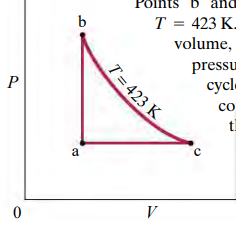
\includegraphics[width=0.3\textwidth]{figures/20-17.png}
\end{figure}
\begin{align*}
    \intertext{Process ab is isovolumetric, which means $W = 0$ and $\Delta
    E_{int} = Q_{in}$} 
    \intertext{Recall that \Delta E_{int} = \frac 3 2 nRT = Q_{in}}
    Q_{in} &= \frac 3 2 (1.0 mol)(8.314 \displaystyle\frac{J}{
        mol \cdot
    K})(423K-273K) \\
        Q_{in} &\approx 1870.65J
    \intertext{Process bc is isothermal and work is done by gas, so $W = nrT\ln (\displaystyle\frac{V_c}{V_b})$ and $Q =
    W$} 
        W &= (1.0mol)(8.314 \displaystyle\frac{J}{mol\cdot
    K})(423K)\ln (\frac ? ?)
    \intertext{Finding $V_f$ and V_0}
    \intertext{At a, we are at STP and using the Ideal Gas Law, we get P_a V_a = nRT}
            V_a &= \displaystyle\frac{nrT}{P_a} =
            \displaystyle\frac{(1.0mol)(8.314 \displaystyle\frac{J}{mol\cdot
            K})(273K)}{1.013\times 10^5 \displaystyle\frac{N}{m^2}} \\
            V_a &\approx 0.0224\;m^3
    \intertext{At c, $P_a = P_c$ so $P= 1.013\times 10 ^5
    \displaystyle\frac{N}{m^2}$ and the process to c was isothermal so $T=423K$}
            V_c &= \displaystyle\frac{nrT}{P} = \displaystyle\frac{(1.0mol)(8.314
    \displaystyle\frac{J}{mol\cdot K})(423K)}{1.013\times 10^5
    \displaystyle\frac{N}{m^2}} \\
                V_c &\approx 0.0347\;m^3
    \intertext{Going back to bc, the work done is}
                W &= (1.0mol)(8.314 \displaystyle\frac{J}{mol\cdot K})(423K)\ln
    (\displaystyle\frac{0.0347\;m^3}{0.0224\;m^3}) \\
                W &\approx 1539J
    \intertext{Process ca is isobaric and has work done on the gas}
                W &= P\Delta V = (1.013\times 10^5 \displaystyle\frac{N}{m^2})(0.0224\;m^3 -
    0.0347\;m^3) \\
                W &\approx -1246J
    \intertext{Finally, the efficiency would be} 
                e &= \displaystyle\frac{W}{Q_{in}} = \displaystyle\frac{1539J -
                1246J}{1870.65J + 1539J} \approx 0.0859\\ 
                e &\approx 8.59\%\;\text{efficiency}
\end{align*}
\newpage
\begin{center}
    \subsection*{\textbf{\textit{20-3 Carnot Engine}}}
\end{center}
\subsubsection*{
    8. What is the maximum efficiency of a heat engine whose
    operating temperatures are 550°C and 365°C?
}
\begin{align*}
    \intertext{Recall, that Carnot efficiency is in Kelvin not Celsius}
    e_{carnot} &= 1 - \displaystyle\frac{T_L}{T_H} = 1 -
    \displaystyle\frac{365\degree C + 273K}{550\degree C + 273K} = 1 -
    \displaystyle\frac{638K}{823K} \\
    e_{carnot} &\approx 22.5\% 
\end{align*} 
\subsubsection*{
    13. A nuclear power plant operates at 65\% of its maximum
    theoretical (Carnot) efficiency between temperatures of 660°C
    and 330°C. If the plant produces electric energy at the rate of
    1.2 GW, how much exhaust heat is discharged per hour?
}
\begin{align*}
    e_{carnot\;max} &= 1 - \displaystyle\frac{603K}{933K} \approx 0.354 \\
    \text{Total Power} &= \displaystyle\frac{\text{Actual Power}}{(max\;
    e)(operating\;e)} = \displaystyle\frac{1.2
    GW}{(0.354)(0.65)} \\
    \text{Total Power} &\approx 5.215 GW \\\\
    \text{Exhaust Power} &= \text{Total Power} - \text{Actual Power} \\
    \text{Exhaust Power} &= 5.215 GW - 1.2GW = 4.015 GW \\\\
    (\displaystyle\frac{4.015 GJ}{1s})(\displaystyle\frac{1.0\times 10^9
J}{1GJ})(\displaystyle\frac{3600s}{1h}) &\approx 1.4\times 10^{13}
\displaystyle\frac{J}{h}
\end{align*}
\subsubsection*{
    14. A Carnot engine performs work at the rate of 520 kW
    with an input of 950 kcal of heat per second. If the
    temperature of the heat source is 560°C, at what temperature
    is the waste heat exhausted?
}
\begin{align*}
    \intertext{Recall that efficiency can either be $1 - 
    \displaystyle\frac{T_L}{T_H}$ or $\displaystyle\frac{W}{Q_{in}}$, so we can
    relate these}
    1 - \displaystyle\frac{T_L}{T_H} &= \displaystyle\frac{W}{Q_{in}} \\
    T_L &= T_H(1 - \displaystyle\frac{W}{Q_{in}}) \\
    \intertext{Adding a variable of time,}
    T_L &= T_H(1 - \displaystyle\frac{\frac{W}{t}}{\frac{Q_{in}}{t}}) =
    (560\degree C + 273K)(1- \displaystyle\frac{520000 \frac{J}{s}}{3976700
    \frac{J}{s}}) \\
    T_L &\approx 724K \;or\;450\degree C
\end{align*}
\subsubsection*{
    17. A heat engine utilizes a heat source at 580°C and has a
    Carnot efficiency of 32\%. To increase the efficiency to 38\%,
    what must be the temperature of the heat source?
}
\begin{align*}
    \intertext{Given that $e_{carnot} = 0.32$ we need to first solve for
    temperature of the waste heat}
    0.32 &= 1 - \displaystyle\frac{T_L}{580\degree C + 273K} \\
    T_L &= (0.32 - 1)(-853K) \\
    T_L &\approx 580K
    \intertext{Assuming $T_L$ will remain the same}
    e_2 &= 1 - \displaystyle\frac{T_L}{T_H} \\
    T_He_2 &= 1 - T_L \\
    T_H(e_2 - 1) &= -T_C \\
    T_H &= \displaystyle\frac{T_C}{1-e_2} = \displaystyle\frac{580K}{1 - (0.38)}
    \\
    T_H &\approx 935K\;or\;662\degree C
\end{align*} 
\newpage
\begin{center}
    \subsection*{\textbf{\textit{20-5 and 20-6 Entropy}}}
\end{center}
\subsubsection*{
    33. A 7.5-kg box having an initial speed of 4.0$\frac m s$ slides
    along a rough table and comes to rest. Estimate the total
    change in entropy of the universe. Assume all objects are at
    room temperature (293 K).
}
\begin{align*}
    \intertext{Entropy is calculated with $\Delta s = \displaystyle\int \displaystyle\frac{dQ}{T}$ and assuming the objects stay at 293K, $\Delta s = \displaystyle\frac{\Delta Q}{T}$}
    \intertext{We know that the box has $KE = \frac 1 2 mv^2 =
    (0.5)(7.5kg)(4.0 \frac{m}{s})^2 = 60J$ of energy}
    \intertext{If the box goes to rest then}
    \Delta E &= 60J - 0J = 60J \\
    \therefore \Delta s &= \displaystyle\frac{\Delta Q}{T} =
    \displaystyle\frac{60J}{293K} \\
    \Delta s &\approx 0.20 \frac{J}{K}
\end{align*}
\subsubsection*{
    34. What is the change in entropy of 1.00 $m^3$ of water at 0°C
    when it is frozen to ice at 0°C?
}
\begin{align*}
    \intertext{Frozen to ice leads me to think we have an increase in
    "organization" which would mean a decrease in entropy}
    \Delta s = \displaystyle\int_{}^{} \displaystyle\frac{dQ}{T} \\
    \intertext{Recall, $Q = mL_f$, $L_f$ being the latent heat of fusion}
    \intertext{This is a phase change so T is constant at 0$\degree$C or 273K, so \Delta s = \displaystyle\frac{\Delta Q}{T}} 
    Q &= (1000kg)(333000 \frac{J}{kg}) = -3.33\times 10^8 J \\
    \therefore \Delta s &= \displaystyle\frac{\Delta Q}{T} =
    \displaystyle\frac{-3.33\times 10^8 J}{273K} \\
    \Delta s &\approx -1.22\times 10^6 J
\end{align*}
\subsubsection*{
    35. If 1.00 $m^3$ of water at 0°C is frozen and cooled to -10$\degree$C 
    by being in contact with a great deal of ice at -10$\degree$C,
    estimate the total change in entropy of the process.
}
\begin{align*}
    \intertext{We need to find and sum the different changes of entropy at the
    different stages of the system}
    \Delta s_1 &= \displaystyle\frac{Q_1}{T_1} = \displaystyle\frac{mL_f}{T_1} =
    \displaystyle\frac{(1000kg)(333000 \displaystyle\frac{J}{kg})}{273K} \\
    \Delta s_1 &\approx -1.21978\times 10^6 \frac{J}{K} \\\\
    \Delta s_2 &= \displaystyle\frac{mc_{ice}\Delta T}{T_2} \qquad [\text{$T_2 =
    T_{avg}$ which is -5$\degree$C or 268K}] \\
    \Delta s_2 &= \displaystyle\frac{(1000kg)(2100
    \displaystyle\frac{J}{kg\cdot K})(273K-263K)}{268K} \\
    \Delta s_2 &\approx -7.8358 \times 10^4 \displaystyle\frac{J}{K}
    \\\\
    \Delta s_3 &= \displaystyle\frac{-Q_1 - Q_2}{T_3} = \displaystyle\frac{mL_f
    + mc_{ice} \Delta T_2}{T_3} \\
    \Delta s_3 &= \displaystyle\frac{(1000kg)(333000
    \displaystyle\frac{J}{kg}) + (1000kg)(2100 \displaystyle\frac{J}{kg\cdot
    K})(273K - 263K)}{-10 + 273K} \\ 
    \Delta s_3 &\approx 1.3460\times 10^6 \displaystyle\frac{J}{K} \\\\
    \Delta s &= \Delta s_1 + \Delta s_2 + \Delta s_3 \\ 
        &= -1.21978\times 10^6 \displaystyle\frac{J}{K} - 7.8358\times 10^4
        \displaystyle\frac{J}{K} + 1.3460\times 10^6
        \displaystyle\frac{J}{K} \\
    \Delta s &\approx 5.0\times 10^4 \displaystyle\frac{J}{K}
\end{align*}
\newpage
\begin{center}
    \subsection*{\textbf{\textit{General Problems}}}
\end{center}
\subsubsection*{
    77. The \textit{Stirling cycle}, shown in Fig. 20–27, is useful to describe
    external combustion engines as well as solar-power systems.
    Find the efficiency of the cycle in terms of the parameters
    shown, assuming a monatomic gas as the working substance. The
    processes \textit{ab} and \textit{cd} are isothermal whereas \textit{bd} and \textit{da} are at constant
    volume. How does it compare to the Carnot efficiency?
}
\begin{figure}[h]
    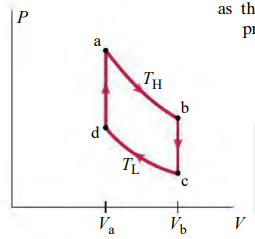
\includegraphics[width=0.3\textwidth]{figures/20-27.png}
\end{figure}
\begin{align*}
    \intertext{Process ab is isothermal so $Q = W$} 
    W_{ab} &= nRT_H \ln (\displaystyle\frac{V_b}{V_a}) = Q_{ab}
    \intertext{Process bc is isovolumetric, so $W = 0$ and $\Delta E_{int} =
    Q_{bc}$}
    Q_{bc} &= \frac 3 2 nR\Delta T = \frac 3 2 nR(T_L - T_H)
    \intertext{Process cd is isothermal and work is done on the gas, so $Q = -W$}
    -W_{cd} &= -1(nRT_L \ln (\displaystyle\frac{V_a}{V_b})) = -nRT_L \ln
    (\displaystyle\frac{V_b}{V_a}) = Q_{cd}
    \intertext{Process da is isovolumetric, so $W = 0$ and $\Delta E_{int} =
    Q_{da}$}
    Q_{da} &= \frac 3 2 nR\Delta T = \frac 3 2 nR(T_H - T_L)
    \intertext{Now to find our Stirling efficiency,}
    e_{Stirling} &= \displaystyle\frac{\sum W}{Q_{in}} =
    \displaystyle\frac{W_{ab} - W_{cd}}{Q_{ab}+Q_{da}} \\
    e_{Stirling} &= \displaystyle\frac{nRT_H\ln (\displaystyle\frac{V_b}{V_a}) - nRT_L\ln
    (\displaystyle\frac{V_b}{V_a})}{nRT_H\ln (\displaystyle\frac{V_b}{V_a})+
    \frac 3 2 nR(T_H - T_L)} \\
    e_{Stirling} &= \displaystyle\frac{(T_H - T_L)\ln
    (\displaystyle\frac{V_b}{V_a})}{T_H\ln (\displaystyle\frac{V_b}{V_a}) +
    \frac 3 2 (T_H - T_L)} \\
    e_{Stirling} &= \left(\displaystyle\frac{T_H -
    T_L}{T_H}\right)\left(\displaystyle\frac{\ln
    (\displaystyle\frac{V_b}{V_a})}{\ln (\displaystyle\frac{V_b}{V_a}) + \frac 3
    2(\displaystyle\frac{T_H - T_L}{T_H})}\right) \\
    \intertext{We see that the Carnot efficiency is}
    e_{carnot} &= 1 - \displaystyle\frac{T_L}{T_H} =
    \displaystyle\frac{T_H - T_L}{T_H} \\
    \intertext{This is the same term in front of our expression for the Stirling
    efficiency, yet the term next to it is less than 1}
    \intertext{\therefore e_{Stirling} < e_{Carnot}}
\end{align*} 
\end{document}
